\begin{name}
	{\tenchude}
	{\tendethi}
	{\tentruong}
	{\thoigian}
\end{name}
\TN
\Opensolutionfile{ans}[ans/ans\currfilebase]
%%%%%-----Câu 1.-----%%%%%
\begin{ex}%[2D1H4-3]%[Lớp 12 - Đề KT GKI - NH 2526 - THPT Việt Đức]%[Nguyễn Đức Tiến]
	\immini[thm]{Đường cong trong hình là đồ thị của hàm số nào dưới đây?
	\choice
	{\True $y= \dfrac{-x^2+1}{x}$}
	{$y=\dfrac{-2x^2+1}{2x+2}$}
	{$y=\dfrac{x^2 -x+1}{x-1}$}
	{$y=x^3-3x^2$}}{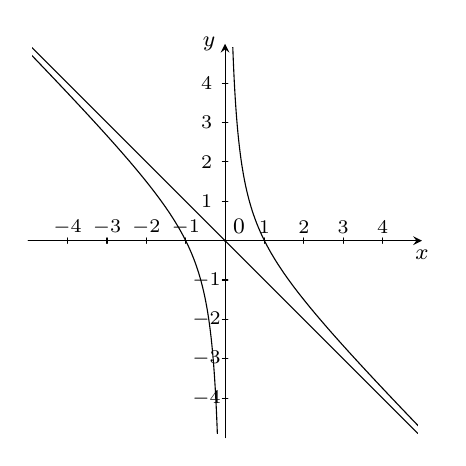
\begin{tikzpicture}[scale=.5,>=stealth, font=\footnotesize, line join=round, line cap=round]
			\def\xmin{-5} \def\xmax{5}
			\def\ymin{-5} \def\ymax{5}
			\draw[->] (\xmin,0)--(\xmax,0) node [below]{$x$};
			\draw[->] (0,\ymin)--(0,\ymax) node [left]{$y$};
			\fill (0,0) circle (1pt) node[shift={(45:2.5mm)}]{$0$};
			\begin{scope}
				\clip (\xmin+0.1,\ymin+0.1) rectangle (\xmax-0.1,\ymax-0.1);
				\draw[black,smooth,samples=300,domain=0.01:\xmax] plot(\x,{(-(\x)^2+1)/(\x)});
				\draw[black,smooth,samples=300,domain=\xmin:-0.01] plot(\x,{(-(\x)^2+1)/(\x)});
				\draw[black,smooth,samples=300,domain=\xmin:\xmax] plot(-\x,{(\x)});
			\end{scope}
			%Vẽ các điểm trên trục Ox
			\foreach \x/\g in {-4/90,-3/90,-2/90,-1/90,1/90,2/90,3/90,4/90}
			\draw[thin] (\x,2pt)--(\x,-2pt) + (\g:4mm) node {\scriptsize $\x$};
			\foreach \y/\g in {-4/180,-3/180,-2/180,-1/180,1/180,2/180,3/180,4/180}
			\draw[thin] (2pt,\y)--(-2pt,\y) + (\g:4mm) node {\scriptsize $\y$};
	\end{tikzpicture}}
	
	
	\loigiai{
		$y= \dfrac{-x^2+1}{x}=-x + \dfrac{1}{x}$.
	}
\end{ex}
%%%%==============HetCau_EX1==============%%%
%%%%==============Cau_EX2==============%%%
\begin{ex}%[2D1H4-1]%[Lớp 12 - Đề KT GKI - NH 2526 - THPT Việt Đức]%[Nguyễn Đức Tiến]
Đường thẳng nào dưới đây là tiệm cận xiên của đồ thị hàm số $y=\dfrac{x^2 -5x +2026}{x-2}$?
\choice
{$y=x+1$}
{$y=x+2$}
{$y=x-2$}
{\True $y=x-3$}
\loigiai
{ $y=\dfrac{x^2 -5x +2026}{x-2}=\dfrac{(x-2)(x-3)+2020}{x-2}= x-3 + \dfrac{2020}{x-2}$ Điều kiện xác định $x\neq 2$.\\
Suy ra
$\lim\limits_{x\to+\infty}[f(x)-(x-3)]=\lim\limits_{x\to + \infty}\left( \dfrac{2020}{x-2}\right) =0$. \\
Do đó $y=x-3$ là tiệm cận xiên của đồ thị hàm số.
}
\end{ex}
%%%%==============HetCau_EX2==============%%%

%%%%==============Cau_EX3==============%%%
\begin{ex}%[2D1H3-3]%[Lớp 12 - Đề KT GKI - NH 2526 - THPT Việt Đức]%[Nguyễn Đức Tiến]
Điểm cực đại của đồ thị hàm số $y= \dfrac{x^2-4x+5}{x-2}$ là
\choice
{$P(2;1)$}
{$Q(1;3)$}
{$M(1;-2)$}
{\True $N(3;2)$}
\loigiai
{Xét $y'=0$
$\Leftrightarrow y' = 1 - \dfrac{1}{(x-2)^2}=0\Rightarrow (x-2)^2 =1\Leftrightarrow \hoac{&x-2 = 1\\&x-2 =-1}\Leftrightarrow \hoac{&x = 3\\&x =1}$.
\begin{center}

\begin{tikzpicture}
	\tkzTabInit[nocadre=false,lgt=1.5,espcl=2,deltacl=0.6]
	{$x$/0.7,$y'$/0.7,$y$/2}{$-\infty$,$1$,$2$, $3$,$+\infty$}
	\tkzTabLine{,-,$0$,+,d,+,$0$,-,}
	\tkzTabVar{+/$+\infty$,-/$-2$,+D-/$+\infty$/$-\infty$,+/$2$,-/$-\infty$}
\end{tikzpicture}
\end{center}
Điểm cực đại của đồ thị hàm số là $N(3;2)$.
}
\end{ex}
%%%%==============HetCau_EX3==============%%%

%%%%==============Cau_EX4==============%%%
\begin{ex}%[2D1N3-1]%[Lớp 12 - Đề KT GKI - NH 2526 - THPT Việt Đức]%[Nguyễn Đức Tiến]
\immini[thm]{
Cho hàm số $y=f(x)$ xác định và liên tục trên $\mathbb{R}$ có đồ thị như hình vẽ bên. Tìm giá trị nhỏ nhất $m$ và giá trị lớn nhất $M$ của hàm số $y=f(x)$ trên đoạn $[-2;2]$.
\choice
{$m=-2; M=2$}
{$m=-5; M=0$}
{$m=-1; M=0$}
{\True $m=-5; M=-1$}}
{
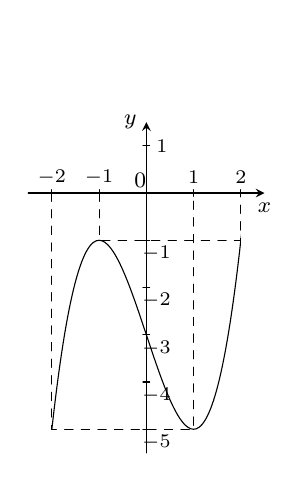
\begin{tikzpicture}[scale=0.6,>=stealth, font=\footnotesize, line join=round, line cap=round]  
	%Vẽ hệ trục
	\draw[->] (-2.5,0)--(2.5,0) node[below]{$x$};
	\draw[->] (0,-5.5)--(0,1.5) node[left]{$y$};
	\node at (0.2,-0.1) [above left]{$0$};
	%Vẽ hàm số
	\begin{scope}
		\clip (-2,-5) rectangle (2,3.5);
		\draw[smooth,domain=-3:3,samples=100]
		plot (\x, {(\x)^3-3*(\x)-3});
	\end{scope}
	%Vẽ các điểm gióng
	\draw[dashed,thin] (-2,0)--(-2,-5)--(1,-5)--(1,0);
	\draw[dashed,thin] (-1,0)--(-1,-1)--(2,-1)--(2,0);
	%Vẽ các điểm trên trục Ox
	\foreach \x/\g in {-2/90,-1/90,1/90,2/90}
	\draw[thin] (\x,2pt)--(\x,-2pt) + (\g:4mm) node {\scriptsize $\x$};
	%Vẽ các điểm trên trục Oy
	\foreach \y/\g in {-5/-45,-4/-45,-3/-45,-2/-45,-1/-45,1/0}
	\draw[thin] (2pt,\y)--(-2pt,\y) + (\g:4mm) node {\scriptsize $\y$};
\end{tikzpicture}
}

\loigiai{
	$m = \min\limits_{[-2;2]}f(x) =-5$.\\
$M = \max\limits_{[-2;2]}f(x) =-1$.

}
\end{ex}
%%%%==============HetCau_EX4==============%%%

%%%%==============Cau_EX5==============%%%
\begin{ex}%[2D1H1-1]%[Lớp 12 - Đề KT GKI - NH 2526 - THPT Việt Đức]%[Nguyễn Đức Tiến]
Trong các hàm số dưới đây, hàm số nào sau đây nghịch biến trên $\mathbb{R}$?
\choice
{\True $y=-x^3-2x-3$}
{$y= \dfrac{x+4}{x-1}$}
{$y=-x^3-3x^2+3$}
{$y=-x^4+2x^2+3$}
\loigiai
{
Xét $y=-x^3-2x-3$.\\
Ta có $y'= -3x^2 -2 $\\
Suy ra hàm số $ y=-x^3-2x-3$ nghịch biến trên $\mathbb{R}$.\\
$y'<0,\, \forall x \in \mathbb{R}$.
}
\end{ex}
%%%%==============HetCau_EX5==============%%%

%%%%==============Cau_EX6==============%%%
\begin{ex}%[2D1N1-2]%[Lớp 12 - Đề KT GKI - NH 2526 - THPT Việt Đức]%[Nguyễn Đức Tiến]
\immini[thm]{
Cho hàm số $y=ax^3 + bx^2 +cx +d$ ($a$, $b$, $c$, $d$ $\in \mathbb{R}, a \neq 0$) có đồ thị là đường cong như hình bên. Hàm số đã cho nghịch biến trên miền nào dưới đây?
\choice
{($-\infty$; $+\infty$)}
{($2;+\infty$)}
{\True ($-1;1$)}
{$(-\infty; 0)$}
}
{
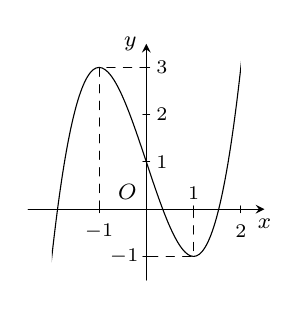
\begin{tikzpicture}[scale=0.6,>=stealth, font=\footnotesize, line join=round, line cap=round]  
	%Vẽ hệ trục
	\draw[->] (-2.5,0)--(2.5,0) node[below]{$x$};
	\draw[->] (0,-1.5)--(0,3.5) node[left]{$y$};
	\node at (0,0) [above left]{$O$};
	%Vẽ hàm số
	\begin{scope}
		\clip (-2,-1.5) rectangle (2,3.5);
		\draw[smooth,domain=-3:3,samples=100]
		plot (\x, {(\x)^3-3*(\x)+1});
	\end{scope}
	%Vẽ các điểm gióng
	\draw[dashed,thin] (1,0)--(1,-1)--(0,-1);
	\draw[dashed,thin] (-1,0)--(-1,3)--(0,3);
	%Vẽ các điểm trên trục Ox
	\foreach \x/\g in {-1/-90,1/90,2/-90}
	\draw[thin] (\x,2pt)--(\x,-2pt) + (\g:4mm) node {\scriptsize $\x$};
	%Vẽ các điểm trên trục Oy
	\foreach \y/\g in {-1/180,1/0,2/0,3/0}
	\draw[thin] (2pt,\y)--(-2pt,\y) + (\g:4mm) node {\scriptsize $\y$};
\end{tikzpicture}
}

\loigiai
{Hàm số nghịch biến trên khoảng $(-1;1)$.}
\end{ex}
%%%%==============HetCau_EX6==============%%%

%%%%==============Cau_EX7==============%%%
\begin{ex}%[2D1V1-2]%[Lớp 12 - Đề KT GKI - NH 2526 - THPT Việt Đức]%[Nguyễn Đức Tiến]
Hàm số $y = x^4 - 8x^2 +2\,025$ đồng biến trên khoảng nào sau đây?
\choice
{$(-\infty; 0)$}
{$(0; + \infty)$}
{\True $(-2;0)$}
{$(-\infty;\infty)$}
\loigiai 
{Tập xác định $\mathscr{D} =\mathbb{R}$.\\
Ta có $y = x^4 - 8x^2 +2\,025$\\
Đạo hàm $y' = 4x^3 - 16x=0$\\
Xét $y'=0\Leftrightarrow \hoac{&4x=0\\&x^2 -4 =0}\Leftrightarrow \hoac{&x=0\\&x =2\\&x=-2}$
\begin{center}

\begin{tikzpicture}
	\tkzTabInit[nocadre=false,lgt=1.5,espcl=2,deltacl=0.6]
	{$x$/0.7,$y'$/0.7,$y$/2}{$-\infty$,$-2$,$0$, $2$,$+\infty$}
	\tkzTabLine{,-,$0$,+,0,-,$0$,+,}
	\tkzTabVar{+/$+\infty$,-/$2\,009$,+/$2\,025$,-/$2\,009$,+/$+\infty$}
\end{tikzpicture}
\end{center}
Hàm số $y = x^4 - 8x^2 +2\,025$ đồng biến trên $(-2;0)$.
}
\end{ex}
%%%%==============HetCau_EX7==============%%%

%%%%==============Cau_EX8==============%%%
\begin{ex}%[2D1N4-1]%[Lớp 12 - Đề KT GKI - NH 2526 - THPT Việt Đức]%[Nguyễn Đức Tiến]
Đường thẳng nào dưới đây là tiệm cận đứng của đồ thị hàm số $y = \dfrac{2x+1}{x+1}$?
\choice
{$y=2$}
{\True $x=-1$}
{$x=1$}
{$y=-1$}
\loigiai
{Hàm số có tập xác định $\mathscr{D} = \mathbb{R} \setminus \{-1\}$, nên tiệm cận đứng là $x=-1$.}
\end{ex}
%%%%==============HetCau_EX8==============%%%

%%%%==============Cau_EX9==============%%%
\begin{ex}%[2D1V4-3]%[Lớp 12 - Đề KT GKI - NH 2526 - THPT Việt Đức]%[Nguyễn Đức Tiến]
\immini[thm]{Cho hàm số bậc ba $y = f(x)$ có bảng biến thiên như sau. Hàm số đã cho là
\choice
	{$f(x) = -x^3 + 3x^2 -2$}
	{$f(x) = x^3 + 3x -2$}
	{$f(x) = \dfrac{x^3}{3} + x^2 -2$}
	{\True $f(x) =x^3 + 3x^2 -2$}
}{
\begin{tikzpicture}
	\tkzTabInit[nocadre=false,lgt=1.5,espcl=2,deltacl=0.6]
	{$x$/0.7,$y'$/0.7,$y$/2}{$-\infty$,$-2$,$0$,$+\infty$}
	\tkzTabLine{,+,0,-,$0$,+,}
	\tkzTabVar{-/$-\infty$,+/$2$,-/$-2$,+/$+\infty$}
\end{tikzpicture}}
	\loigiai
	{
	Xét $f(x) = ax^3 + bx^2 + cx +d $. Suy ra $f'(x) = 3ax^2 + 2bx + c =0$.\\
	$\heva{&-8a +4b -2c +d =2\\&d=0\\&12a-4b+c=0\\&c=0}$$\Rightarrow$$\heva{&a=1\\&b=3\\&c=0\\&d=-2}$.\\
	$\Rightarrow f(x)=x^3 + 3x^2 -2$.
	}
\end{ex}
%%%%==============HetCau_EX9==============%%%

%%%%==============Cau_EX10==============%%%
\begin{ex}%[2D1N2-2]%[Lớp 12 - Đề KT GKI - NH 2526 - THPT Việt Đức]%[Nguyễn Đức Tiến]
\immini[thm]{Cho hàm số $y=f(x)$ có bảng biến thiên như sau. Hàm số đã cho đạt cực đại tại điểm nào sau đây?
\choice
	{$x=2$}
	{$x=-1$}
	{\True $x=1$}
	{$x=0$}
}
	{
\begin{tikzpicture}
		\tkzTabInit[nocadre=false,lgt=1.5,espcl=2,deltacl=0.6]
		{$x$/0.7,$y'$/0.7,$y$/2}{$-\infty$,$1$,$2$,$+\infty$}
		\tkzTabLine{,+,0,-,$0$,+,}
		\tkzTabVar{-/$-\infty$,+/$0$,-/$-1$,+/$+\infty$}
	\end{tikzpicture}}
\end{ex}
%%%%==============HetCau_EX10==============%%%

%%%%==============Cau_EX11==============%%%
\begin{ex}%[2D1H3-3]%[Lớp 12 - Đề KT GKI - NH 2526 - THPT Việt Đức]%[Nguyễn Đức Tiến]
Giá trị cực tiểu của hàm số $y = -x^4 + 8x^2 + 2\,025$ là bao nhiêu?
\choice
{$y=2\,041$}
{$y=0$}
{$ y= -2\,025$}
{\True $y=2\,025$}
\loigiai {
Tập xác định $\mathscr{D} =\mathbb{R}$.\\
Ta có $y = -x^4 + 8x^2 +2\,025$\\
Đạo hàm $y' = -4x^3 + 16x=0$\\
$y'=0 \Leftrightarrow \hoac{&-4x=0\\&x^2 -4 =0} \Leftrightarrow \hoac{&x=0\\&x =2\\&x=-2}$.
\begin{center}
	
\begin{tikzpicture}
		\tkzTabInit[nocadre=false,lgt=1.5,espcl=2,deltacl=0.6]
		{$x$/0.7,$y'$/0.7,$y$/2}{$-\infty$,$-2$,$0$, $2$,$+\infty$}
		\tkzTabLine{,-,$0$,+,0,-,$0$,+,}
		\tkzTabVar{-/$-\infty$,+/$2\,041$,-/$2\,025$,+/$2\,041$,-/$-\infty$}
	\end{tikzpicture}
\end{center}
	Vậy giá trị cực tiểu của hàm số là $y = 2\,025$.
}
\end{ex}
%%%%==============HetCau_EX11==============%%%
%%%%==============Cau_EX12==============%%%
\begin{ex}%[2D1H3-1]%[Lớp 12 - Đề KT GKI - NH 2526 - THPT Việt Đức]%[Nguyễn Đức Tiến]
Giá trị lớn nhất của hàm số $y= \sqrt{4x -x^2}$ trên $[0;4]$ là
\choice
{\True $2$}
{$4$}
{$0$}
{$1$}
\loigiai 
{
	Tập xác định của hàm số là $\mathscr{D} = [0; 4]$.\\
Ta có đạo hàm
$$ y' = \dfrac{(4x - x^2)'}{2\sqrt{4x - x^2}} = \dfrac{4 - 2x}{2\sqrt{4x - x^2}} = \dfrac{2 - x}{\sqrt{4x - x^2}} $$
Cho $y' = 0 \Leftrightarrow 2 - x = 0 \Leftrightarrow x = 2$.
\begin{center}
	
\begin{tikzpicture}
		\tkzTabInit[nocadre=false,lgt=1.5,espcl=2,deltacl=0.6]
		{$x$/0.7,$y'$/0.7,$y$/2}{$0$,$2$,$4$}
		\tkzTabLine{0,+,0,-,0}
		\tkzTabVar{-/$0$,+/$2$,-/$0$}
	\end{tikzpicture}
\end{center}
$\Rightarrow \max\limits_{[0;4]}y = 2$.
}
\end{ex}


%%%%==============HetCau_EX12==============%%%
\TNTF
%%%==============Cau_EX1==============%%%
\begin{ex}%[2D1V3-6]%[Lớp 12 - Đề KT GKI - NH 2526 - THPT Việt Đức]%[Nguyễn Đức Tiến]
Để kỷ niệm $70$ năm ngày thành lập trường THPT X, các cựu học sinh tổ chức phát hành áo kỷ niệm gây quỹ học bổng. Giả sử doanh số (tính bằng số áo bán được) tuần theo quy luật logistic được mô hình hóa bằng hàm số $f(t)=\dfrac{7\,000}{1+69e^{-t}}, t \ge 0$, trong đó thời gian $t$ được tính theo đơn vị ngày, kể từ thời điểm ngày phát hành đầu tiên (ngày 11/8/2\,025).
\choiceTF
{Sau ba ngày kể từ thời điểm ngày phát hành đầu tiên, số áo bán ra vượt quá $2\,000$ chiếc}
{\True Tổng số áo được bán ra không vượt quá $7\,000$ chiếc}
{\True Ngay tại thời điểm ngày phát hành đầu tiên, số áo được bán ra đã đạt $100$ chiếc}
{Đạo hàm $f'(t)$ sẽ biểu thị tốc độ phát hành. Sau $360$ giờ kể từ thời điểm phát hành đầu tiên thì tốc độ phát hành là lớn nhất}
\loigiai 
{$$f(t)=\dfrac{7\,000}{1+69e^{- t}}, t \ge 0 \Rightarrow f'(t) = \dfrac{483\,000e^{-t}}{(1 + 69e^{-t})^2}$$
\begin{itemchoice}
\itemch $f(3)=1\,578 < 2\,000$.
\itemch $$\lim_{t\to\infty} 69\cdot e^{-t} = 0$$\\$$\Rightarrow \lim_{t\to\infty}f(t)= \dfrac{7\,000}{1 + \lim_{t\to\infty} 69\cdot e^{-t}} = 7\,000.$$
\itemch $$f(0)=\dfrac{7\,000}{1+69e^{- 0}}=\dfrac{7\,000}{70}=100.$$
\itemch $360$ giờ = $15$ ngày, khác với thời điểm tốc độ phát hành lớn nhất $t=\ln(69)\approx 4{,}234$ ngày.
Ta có 
$$ f'(t) = \dfrac{483\,000e^{-t}}{(1 + 69e^{-t})^2}$$
Đạo hàm cấp hai của hàm số Logistic là:
$$f''(t) = \dfrac{483\,000e^{-t} (69e^{-t} - 1)}{(1 + 69e^{-t})^3}$$
Để tìm giá trị $t$ mà tại đó tốc độ phát hành là lớn nhất, ta giải phương trình $f''(t) = 0$\\
$\dfrac{483\,000e^{-t} (69e^{-t} - 1)}{(1 + 69e^{-t})^3} = 0$\\
$69e^{-t} - 1 = 0$\\
$e^{-t} = \dfrac{1}{69}$\\
$\ln(e^{-t}) = \ln\left(\dfrac{1}{69}\right)$\\
$\Rightarrow t = \ln(69) \approx 4{,}234\, \text{ngày}$.
\end{itemchoice}
}
\end{ex}
%%%==============Cau_EX2==============%%%
\begin{ex}%[2D1H4-3]%[Lớp 12 - Đề KT GKI - NH 2526 - THPT Việt Đức]%[Nguyễn Đức Tiến]
Cho hàm số $y = g(x)$ có bảng biến thiên như hình vẽ sau
\begin{center}
\begin{tikzpicture}[line join = round, line cap=round,>=stealth,font=\normalsize,scale=1]
	\draw (0,0)--(10,0);
	\draw (0,-1)--(10,-1);
	\draw 
	(0.5,0)node[above]{$x$}
	(0.5,-0.75)node[above]{$g\rq(x)$}
	(0.5,-2)node[above]{$g(x)$}
	(1.4,0)node[above]{$-\infty$}
	(3.4,0)node[above]{$-2$}
	(7,0)node[above]{$0$}
	(9.7,0)node[above]{$+\infty$}
	(5.2,-0.75)node[above]{$+$}
	(8.35,-0.75)node[above]{$-$}
	(3.45,-2.9)node[right]{$0$}
	(6.98,-1)node[below left]{$+\infty$}
	(7,-1)node[below right]{$1$}
	(9.7,-3)node{$-\infty$}
	;
	\draw(1,0.5)--(1,-3)
	(3.49,0)--(3.49,-3)
	(3.53,0)--(3.53,-3)
	(6.98,0)--(6.98,-3)
	(7.02,0)--(7.02,-3)
	;
	\fill[pattern=north east lines] (1,0)rectangle (3.49,-3);
	\draw[->](3.75,-2.8)--(6.38,-1.4);
	\draw[->](7.4,-1.4)--(9.4,-2.8);
\end{tikzpicture}
\end{center}
\choiceTF
{\True Hàm số $y = g(x)$ nghịch biến trên $(0;+\infty)$}
{Hàm số $y=g(x)$ đạt cực đại tại $x=0$}
{\True Đồ thị hàm số $y=g(x)$ luôn cắt trục hoành tại ít nhất một điểm}
{Đồ thị hàm số $y = \dfrac{1}{g(x) -1}$ có $x=a$ đường tiệm cận đứng và $y=b$ đường tiệm cận ngang. Khi đó $a^2 + b^2 =10$}
\loigiai
{d) $x=a$ là tiệm cận đứng \\
$g(x)-1=0 \Rightarrow -2 \le a < 0$\\
$\lim \limits_{x \to +\infty} g(x)=-\infty \Rightarrow \lim \limits_{x \to +\infty} y=0=b$ \\
$\Rightarrow a^2 + b^2 < 10$
}
\end{ex}
%%%==============Cau_EX3==============%%%
\begin{ex}%%[2D1H2-1]%[Lớp 12 - Đề KT GKI - NH 2526 - THPT Việt Đức]%[Nguyễn Đức Tiến]
	Cho hàm số $y=f(x)=x^3-3x^2-9x$. 
	\choiceTF
	{\True Đồ thị hàm số $y=f(x)$ có hai điểm cực trị nằm về hai phía của trục tung}
	{\True Hàm số $y=f(x)$ có đạo hàm $y'=f'(x)=3x^2-6x-9$ }
	{\True Đường thẳng qua hai điểm cực trị của đồ thị hàm số $y=f(x)$ có hệ số góc là $k=-8$ }
	{Giá trị lớn nhất của hàm số $y=f(x)$ trên đoạn $[0;5]$ bằng $-5$ }
	\loigiai{Tập xác định $\mathscr{D}=\mathbb{R}$.\\
		Ta có $f'(x)=3x^2-6x-9=3(x^2-2x-3)=3(x-3)(x+1)$.\\
		Bảng biến thiên:\\
		\begin{center}
			
\begin{tikzpicture}
				\tkzTabInit[nocadre=true,lgt=1,espcl=3,deltacl=0.5]
				{$x$/0.7,$y'$/0.7,$y$/2}
				{$-\infty$,$-1$,$3$,$+\infty$}
				\tkzTabLine{,-,0,+,0,-,}
				\tkzTabVar{+/$+\infty$,-/$5$,+/$-27$,-/$-\infty$}
			\end{tikzpicture}
		\end{center}
		
		\begin{itemchoice}
			\itemch \textbf{Đúng}.
			Suy ra hàm số có cực đại tại $x=-1$ và cực tiểu tại $x=3$, hai điểm nằm hai phía trục tung.  
			\itemch \textbf{Đúng}.
			Ta có $f'(x)=3x^2-6x-9=3(x^2-2x-3)=3(x-3)(x+1)$.
			\itemch \textbf{Đúng}.
			Tọa độ hai điểm cực trị của đồ thị hàm số là $A(-1;5)$ và $B(3;-27)$.\\
			Hệ số góc của đường thẳng $AB$ là $k=\dfrac{-27-5}{3-(-1)}=-8$.
			\itemch \textbf{Sai}.
			Ta có $f(0)=0$, $f(5)=125-75-45=5$ và $f(3)=27-27-27=-27$.\\
			Vậy giá trị lớn nhất của hàm số $y=f(x)$ trên $[0;5]$ bằng $5$.
	\end{itemchoice}}
\end{ex}
%%%==============Cau_EX4==============%%%
\begin{ex}%[2D1H4-1]%[Lớp 12 - Đề KT GKI - NH 2526 - THPT Việt Đức]%[Nguyễn Đức Tiến]
	Cho hàm số $y=h(x)=\dfrac{x^2-2x-1}{x+1}$.
	\choiceTF
	{Khoảng cách giữa hai điểm cực trị của đồ thị hàm số $y=h(x)$ bằng $10$ }
	{\True $\lim_{x\to +\infty}h(x)=+\infty$}
	{\True Đồ thị hàm số $y=h(x)$ và đường thẳng $(d): y=-2x$ có hai điểm chung phân biệt }
	{\True Đồ thị hàm số $y=h(x)$ có tiệm cận xiên là đường thẳng $(\Delta): y=x-3$  }
	\loigiai{Tập xác định $\mathscr{D}=\mathbb{R}\backslash\{-1\}$.\\
		Ta có $h(x)=\dfrac{x^2-2x-1}{x+1}=x-3+\dfrac{2}{x+1}$.\\
		$h'(x)=1-\dfrac{2}{(x+1)^2}=0 \Rightarrow (x+1)^2=2 \Rightarrow x=-1\pm \sqrt{2}$.
		\begin{itemchoice}
			\itemch \textbf{Sai}.\\
			Hai điểm cực trị của đồ thị hàm số là $A(-1-\sqrt{2};-2\sqrt{2}-4) $ và $B(-1+\sqrt{2};2\sqrt{2}-4)$.\\
			Khoảng cách giữa hai điểm cực trị là $$AB=\sqrt{\left(2 \sqrt{2}\right)^2+\left( 4 \sqrt{2}\right)^2}=\sqrt{8+32}=\sqrt{40}=2 \sqrt{10}.$$
			\itemch \textbf{Đúng}.
			$ \lim\limits_{x\to+\infty}h(x)=\lim\limits_{x\to+\infty}\left(x\cdot\dfrac{1-\dfrac{2}{x}-\dfrac{1}{x^2}}{1+\dfrac{1}{x}} \right) =+\infty$ \\vì  $\heva{&\lim_{x\to+\infty}x=+\infty\\&\lim_{x\to+\infty}\dfrac{1-\dfrac{2}{x}-\dfrac{1}{x^2}}{1+\dfrac{1}{x}}=1>0.}$
			\itemch \textbf{Đúng}.
			Xét phương trình hoành độ giao điểm $x-3+\dfrac{2}{x+1}=-2x \Leftrightarrow
			\hoac{&x=\dfrac{\sqrt{3}}{3}\\&x=-\dfrac{\sqrt{3}}{3}.}$\\
			Phương trình có hai nghiệm phân biệt nên đồ thị hàm số $y=h(x)$ và đường thẳng $(d): y=-2x$ có hai điểm chung phân biệt.
			\itemch \textbf{Đúng}.
			Từ khai triển trên, tiệm cận xiên là $y=x-3$.
	\end{itemchoice}}
\end{ex}
\TNSA
% Câu 1
\begin{ex}%[2D1V3-6]%[Lớp 12 - Đề KT GKI - NH 2526 - THPT Việt Đức]%[Trịnh Văn Cảnh]
	\immini[thm]{Một đường dây điện được nối từ một nhà máy điện ở $A$ đến một hòn đảo ở $C$ (như hình vẽ). 
		Biết $BC=4$ km là khoảng cách từ đảo $C$ đến bờ biển $AB$. Bờ biển $AB$ có độ dài là $10$ km. Tổng chi phí lắp đặt cho $1$ km dây điện trên biển là $50$ triệu đồng, còn chi phí lắp đặt cho $1$ km dây điện trên đất liền là $30$ triệu đồng. Người ta xác định được vị trí điểm $M$ trên đoạn $AB$ là điểm nối dây từ đất liền ra đảo sao cho tổng chi phí lắp đặt là nhỏ nhất. Tính khoảng cách $BM$ (\textit{Đơn vị: km, kết quả làm tròn đến hàng đơn vị}).}{\begin{tikzpicture}[font=\footnotesize,line join=round, line cap=round, >=stealth,scale=0.5] 
			\path 
			(0,0) coordinate (B)
			(9,0) coordinate (A)	
			(3,0) coordinate (M)
			(0,6) coordinate (C)		
			;
			\draw (M)--(C)--(A)--(B)--(C)--(A) ;
			\foreach \x/\pos in{A/50,B/-150,C/90,M/-60}
			\fill (\x) circle(1pt) node[{shift=(\pos:0.25)}]{$\x$}; 
	\end{tikzpicture}}
	\shortans{3}
	\loigiai{Đặt $BM = x$, $(0 \le x \le 10)$.\\
		Khi đó $CM = \sqrt{16 + x^2}$, $AM = 10 - x$.\\
		Ta có hàm tổng chi phí (đơn vị triệu đồng) là \\
		$f(x) = 50\cdot CM + 30\cdot AM = 50\cdot\sqrt{16 + x^2} + 30\cdot(10 - x)$.\\
		Khi đó $f'(x) = \dfrac{50x}{\sqrt{16 + x^2}} - 30$.\\
		Ta có $f'(x) = 0 \Leftrightarrow x = 3$.\\
		Bảng biến thiên
		\begin{center}
			
\begin{tikzpicture}[>=stealth]
				\tkzTabInit[nocadre=true,lgt=1.3,espcl=3,deltacl=0.5]{$x$/.7 ,$f'(x)$/.7,$f(x)$/3}
				{$0$ , $3$ , $10$}
				\tkzTabLine{ , - , $0$ , + , }
				\tkzTabVar{+/$f(0)$ , -/$f(3)$ , +/$f(10)$}
			\end{tikzpicture}
		\end{center}
		Từ bảng biến thiên ta có: $\min\limits_{[0;10]}f(x)=f(3)$.\\
		Vậy $BM = 3$ km.}
\end{ex}

% Câu 2
\begin{ex}%[2D1V3-6]%[Lớp 12 - Đề KT GKI - NH 2526 - THPT Việt Đức]%[Trịnh Văn Cảnh]
	Công ty Apple đề xuất giá bán mỗi chiếc iPhone 17 Pro Max 1TB cho đại lý tại Việt Nam khi đại lý này nhập $x$ chiếc là $P(x)=50\,000\,000-5\,000x$ (VND). Hỏi doanh thu tối đa mà công ty Apple nhận được từ đại lý này là bao nhiêu? (\textit{Đơn vị tỷ VND, kết quả làm tròn đến hàng phần nguyên}).
	\shortans{125}
	\loigiai{Doanh thu (tổng tiền Apple thu được) khi bán $x$ chiếc là:
		$$R(x)=x \cdot P(x)=x(50\,000\,000-5\,000x)=50\,000\,000x-5\,000x^2.$$
		Ta thấy $R(x)$ là hàm bậc hai, có hệ số $-5\,000<0$ nên có giá trị lớn nhất tại $x=-\dfrac{b}{2a}=5\,000$.\\
		Vậy doanh thu tối đa bằng $R(5\,000)=125\,000\,000\,000\text{ VND }=125\text{ tỉ VND}.$\\
		
	}
\end{ex}

% Câu 3
\begin{ex}%[2D1V1-3]%[Lớp 12 - Đề KT GKI - NH 2526 - THPT Việt Đức]%[Trịnh Văn Cảnh]
	Tính tổng các giá trị nguyên dương của tham số $m$ để hàm số $y=x^3-3mx^2+3(3m+4)x+2\,025$ đồng biến trên $(2;+\infty)$.	
	\shortans{10}
	\loigiai{Tập xác định $\mathscr{D}=\mathbb{R}$.\\
		Ta có $y'=3x^2-6mx+3(3m+4)=3\left(x^2-2mx+3m+4\right)
		$.\\
		Đặt $g(x)=x^2-2m x+3m+4$.\\
		Hàm số $y$ đồng biến trên $(2 ;+\infty)$ khi và chỉ khi $g(x) \geq 0, \forall x>2$.\\
		Bảng biến thiên của hàm số $y=g(x)$
		\begin{center}
			
\begin{tikzpicture}
				\tkzTabInit[nocadre=true,lgt=1,espcl=3,deltacl=0.5]
				{$x$/0.7,$y$/2}
				{$-\infty$,$m$,$+\infty$}
				\tkzTabVar{+/$+\infty$,-/$-m^2+3m+4$,+/$+\infty$}
			\end{tikzpicture}
		\end{center}
		\begin{itemize}
			\item \textbf{Trường hợp 1:} $m \leq 2$.\\
			Khi đó $\forall x>2 $ thì $g(x)>g(2)=8-m$.\\
			Để $g(x) \geq 0, \forall x>2$ thì điều kiện là $$g(2) \geq 0 \Leftrightarrow 8-m \geq 0 \Leftrightarrow m \leq 8.$$
			Kết hợp với $m \leq 2$ và $m\in \mathbb{Z^+} $ suy ra $m\in\{1;2\} $.
			\item \textbf{Trường hợp 2:} $m > 2$.\\
			Khi đó $\forall x>2 $ thì $g(x)>g(m)=-m^2+3m+4$.\\
			Để $g(x) \geq 0, \forall x>2$ thì điều kiện là $$-m^2+3 m+4 \geq 0 \Leftrightarrow m^2-3 m-4 \leq 0 \Leftrightarrow-1 \leq m \leq 4. $$
			Kết hợp với $m > 2$ và $m\in \mathbb{Z^+} $ suy ra $m\in\{3;4\} $.
		\end{itemize}
		Vậy $m\in\{1;2;3;4\} $. Tổng các giá trị đó là $1+2+3+4=10$.
	}
\end{ex}

% Câu 4
\begin{ex}%[2D1H2-1]%[Lớp 12 - Đề KT GKI - NH 2526 - THPT Việt Đức]%[Trịnh Văn Cảnh] 
	Tìm giá trị cực tiểu của hàm số $y=x^3+6x^2-15x+2\,033$.	
	\shortans{2025}
	\loigiai{Tập xác định $\mathscr{D}=\mathbb{R}$.\\
		Ta có
		$y'=3x^2+12x-15=3\left(x^2+4 x-5\right)=3(x+5)(x-1) \Leftrightarrow \hoac{&x+5=0\\&x-1=0}\Leftrightarrow\hoac{&x=-5\\&x=1}$.\\
		Bảng biến thiên:\\
		\begin{center}
			
\begin{tikzpicture}
				\tkzTabInit[nocadre=true,lgt=1,espcl=3,deltacl=0.5]
				{$x$/0.7,$y'$/0.7,$y$/2}
				{$-\infty$,$-5$,$1$,$+\infty$}
				\tkzTabLine{,+,0,-,0,+,}
				\tkzTabVar{-/$-\infty$,+/$2\,133$,-/$2\,025$,+/$+\infty$}
			\end{tikzpicture}
		\end{center}
		Từ bảng biến thiên ta có giá trị cực tiểu của hàm số là $2\,025$.}
\end{ex}
%%%==============Bai_BT5==============%%%
\begin{ex}%[2D1C3-5]%[Lớp 12 - Đề KT GKI - NH 2526 - THPT Việt Đức]%[Nguyễn Đức Tiến]	
Cho hàm số $y = f(x) = \dfrac{\cos x + m^2 + 3m}{\cos x + 2}$ ($m$ là tham số thực). Hàm số $y = f(x)$ đạt giá trị lớn nhất trên đoạn $[0; \pi]$ là $M$. Có bao nhiêu giá trị nguyên của tham số $m$ thỏa $M \le -1$.
\shortans{$0$}
\loigiai
{ Ta có đạo hàm:

	\begin{eqnarray*}
		f'(x) &= \dfrac{(-\sin x)(\cos x + 2) - (-\sin x)(\cos x + m^2 + 3m)}{(\cos x + 2)^2} \\
		&= \dfrac{\sin x (m^2 + 3m - 2)}{(\cos x + 2)^2}
	\end{eqnarray*}

	Xét phương trình $f'(x) = 0 \Leftrightarrow \sin x \cdot (m^2 + 3m - 2) = 0$.
	
	\textbf{Trường hợp 1:} $m^2 + 3m - 2 = 0$.
	Khi đó $f'(x) = 0, \forall x$. Hàm số là hàm hằng $f(x) = 1$.
	Vì $1 > -1$ nên trường hợp này loại.
	
	\textbf{Trường hợp 2:} $m^2 + 3m - 2 \ne 0$.
	Khi đó $f'(x) = 0 \Leftrightarrow \sin x = 0 \Leftrightarrow \hoac{&x=0\\&x=\pi}$ (vì $x \in [0; \pi]$).\\
	Ta tính giá trị tại hai đầu mút
	$\heva{&f(0) = \dfrac{1 + m^2 + 3m}{1+2} = \dfrac{m^2 + 3m + 1}{3}\\& f(\pi) = \dfrac{-1 + m^2 + 3m}{-1+2} = m^2 + 3m - 1}$\\
	Vì $\sin x > 0$ trên $(0; \pi)$ nên dấu của $f'(x)$ phụ thuộc vào $A = m^2 + 3m - 2$.
	\begin{enumerate}
		\item Nếu $A > 0$ (hàm đồng biến): $M = f(\pi)$.
		 $M \le -1 \Leftrightarrow m^2 + 3m - 1 \le -1 \Leftrightarrow m^2 + 3m \le 0 \Leftrightarrow m \in [-3; 0]$.\\
		Giao với điều kiện $A > 0$: Thử các giá trị nguyên $m \in \{-3; -2; -1; 0\}$ vào $A = m^2 + 3m - 2$ đều thấy $A < 0$ (vô lý). $\Rightarrow$ Loại.
		\item Nếu $A < 0$ (hàm nghịch biến): $M = f(0)$.\\
$M \le -1 \Leftrightarrow \dfrac{m^2 + 3m + 1}{3} \le -1 \Leftrightarrow m^2 + 3m + 4 \le 0$ (Vô nghiệm).
	\end{enumerate}
Vậy không tồn tại giá trị nguyên nào của $m$ thỏa mãn.
}
\end{ex}
%%%=== ===========HetBai_BT5==============%%%
%%%==============Bai_BT6==============%%%
\begin{ex}%[2D1C4-2]%[Lớp 12 - Đề KT GKI - NH 2526 - THPT Việt Đức]%[Nguyễn Đức Tiến]
Cho hàm số $y = f(x) = \dfrac{ax^2 + bx + 2\,025}{x + 2}$ ($a, b$ là các tham số thực, $a \ne 0$). Biết đồ thị hàm số $y = f(x)$ có một đường tiệm cận xiên $(\Delta): y = x + 4$. Tính giá trị của biểu thức $P = a^2 + b^2$ (kết quả làm tròn đến hàng đơn vị).
\shortans{$37$}
\loigiai 
{
$$ f(x) = \dfrac{ax(x+2) + (b-2a)(x+2) + 2\,025 - 2b + 4a}{x+2} = ax + b - 2a + \dfrac{4a - 2b + 2\,025}{x + 2}.$$
Khi đó, ta có
$$ \lim\limits_{x \to \infty} [f(x) - (ax + b - 2a)] = \lim\limits_{x \to \infty} \dfrac{4a - 2b + 2\,025}{x + 2} = 0.$$
Do đó, đồ thị hàm số nhận đường thẳng $d: y = ax + b - 2a$ làm tiệm cận xiên.\\
Theo giả thiết, tiệm cận xiên là đường thẳng $(\Delta): y = x + 4$.\\
Đồng nhất hệ số của $d$ và $(\Delta)$, ta có hệ phương trình
$$\heva{&a = 1 \\ &b - 2a = 4}\Leftrightarrow \heva{ &a = 1 \\ &b = 4 + 2(1) = 6}.$$
Vậy $P = a^2 + b^2 = 1^2 + 6^2 = 37$.
}
\end{ex}
%%%==============HetBai_BT6==============%%%
\Closesolutionfile{ans}

%%%==============HetBai_BT3==============%%%